
\documentclass[12pt,fleqn,leqno,letterpaper]{article}
\usepackage[utf8]{inputenc}
\usepackage[english]{babel}

\usepackage{hyperref}
\usepackage{graphicx}
\usepackage{minted}

\usepackage{tikz}
\usetikzlibrary{shapes.geometric,positioning}

\include{preamble}


\title{Assignment 2}
\author{Anders L. Hurum\\
    \small{Development of Real-Time Systems}\\
    \small{EIT Digital}\\
    \small{\texttt{andershurum@gmail.com}}
}
\date{September 17, 2017}

\begin{document}


    \maketitle

    \begin{abstract}
        
        The second assignment for the Real-Time systems course consisted of developing 
        an application for exploring how priorities, executiontime, periods influence eachother
        in practise in a Real-Time system. \\ \\
        For more details on the assignment, see the \texttt{assignment\_2.md} document 
        in the repository at github. \\
        
        \url{http://github.com/peakbreaker/tuts\_FreeRTOS}

    \end{abstract}

    \newpage

    \section*{Introduction}
    To fullfill the requirements by the assignment it is planned to implement the RTOS
    with three tasks: 

    \begin{itemize}
        \item prioritysettask
        \item matrixtask
        \item communicationtask 
    \end{itemize} 

    The idea is that matrixtask will be responsible charge of matrix calculations, while 
    communicationstask will handle communication to a peripheral (like transmitting the calculations from matrixtask).
    Finally prioritysettask will measure and manage the tasks, and set priorities according to the requirements
    of our application. \\

    \begin{figure}[h] 
        \centering
        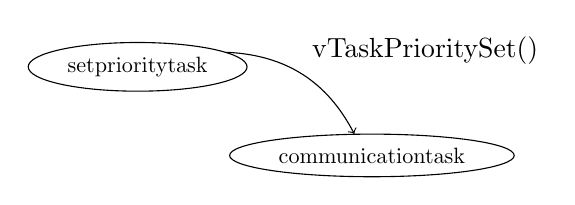
\begin{tikzpicture}
                \node (l1) [ellipse, draw=black, fill=white!20, text=black, scale=0.8]{
                setprioritytask};
                \node (l3) [ellipse, draw=black, fill=white!20, text=black, scale=0.8, below right=1cm of l1]{
                communicationtask};
            \draw[bend left,->]  (l1) to node [auto] {vTaskPrioritySet()} (l3);
        \end{tikzpicture}
        \caption{Tasks}
        \label{figure:tasks}
    \end{figure}

    We aim with this to answer questions relating to execution priorities in FreeRTOS, 
    and find out how priorities, periods and pre-emptiveness influence the behavior of
    execution in Real Time systems.

    \section*{Code}

        Worth noting here is that the main function must pass the handlers of the 
        matrixcalctulation and commun
        icationtask to the prioritysettask so that it can'
        access the tasks.  In doing this we are also doing checks to make sure everything
        went well in setting up the tasks.  thus we implemented the following main procedure: \\

        \begin{minted}{c}
            int main(void)
            {
                
            }
        \end{minted}

        Since we were given the matrixcalculation task and communicationtask, we will simply
        look here at how we implemented the prioritysettask:

        \begin{minted}{c}
            
        \end{minted}

        Note here the use of ... \\

        There was done no changes to the tasks given in the assignment. 
        They were therefore implemented in their own file to reduce clutter and make the code easier to read
    
    \newpage
    \section*{Results}

        The resulting output from the program were as follows : \\

        \begin{figure}[h]
            \centering
            \includegraphics[width=\textwidth]{Debug.png}
            \caption{Debug output}
            \label{figure:debug}
        \end{figure}

        As the output shows, \\
        
        The repository for the entire assignment can be found at my github : \\
        
        \url{http://github.com/peakbreaker/tuts\_FreeRTOS}

        \section*{What did we learn?}

    \end{document}